\chapter{Bayesian Concept Drift Detection} \label{chapt:BDD}

In this chapter we explore Bayesian approaches to concept drift detection. Section \ref{BDD:motivation} motivates a Bayesian approach to concept drift detection. Section \ref{BDD:bddm} introduces Bayesian drift detection method (BDDM), an algorithm for computing posteriors probabilities of concept drift. Section \ref{BDD:BWAF} introduces Bayes with adaptive forgetfulness (BWAF), an efficient method for approximating posterior probabilities of concept drift. Section \ref{BDD:conclusion} summarises this chapter and discusses future work.

%-------------------------------------------------------------------
% MOTIVATION
%-------------------------------------------------------------------

\section{Motivation} \label{BDD:motivation}

In this chapter we consider methods for deriving a posterior probability distribution over concept drift locations, and of the current error rate of the model. We claim that such a derivation is valuable for many practical data science applications where a human is in the loop and there are strict requirements on performance. As illustration, we return to our motivating example of GP referrals triage. The details of this description are fictional.
\begin{displayquote}
    A model has been trained to predict triage labels for GP referrals documents. A drift detector is has been installed to detect when the error rate of the model increases, at which point it will alert a data scientist that the model requires retraining.   
    
    Suppose the data scientist receives an alert that the error rate of the model has increased. The data scientist now has to decide 1) whether the model really requires retraining, and if so 2) how far back in time should the new training data extend so that the new model is trained only on post-drift instances.
    
    The model is required to have an error rate of at most 5\%, or it is not considered fit for purpose. The cost of retraining the model is \$500, as it requires the data scientist to spend several days on site collecting data, and retraining the new model, validating the new model, and deploying the new model. The cost of keeping a model which is not fit for purpose deployed is estimated at \$5000 due to errors in the triage support  leading to inefficient allocation of medical staff. If $\Pr(err>0.05)$ is the probability that the error rate is greater than 5\%, then it is worthwhile retraining the model as long as 
    \begin{equation}
        \Pr(err>0.05) \times \$5000 > \left( 1-\Pr(err>0.05) \right) \times \$500.
    \end{equation}
    This illustrates that it is not only important for the data scientist to know that the error rate has probably increased, but to also have a probability distribution over {\it how much} it has increased. 
    
    If the data scientist has access to a posterior probability distribution over possible error rates at the current time, as in Figure \ref{fig:posterior_rates}, then they can make a more informed decision about whether the model requires retraining or not.   
    
    Let us suppose the data scientist decides that the model {\it does} require retraining. They must now decide which data to use to retrain the model. Other things being equal, the data scientist would like to use more data rather than less so that the model will generalise better. However, the less recent the data, the more likely it is to have become outdated by the concept drift.
    
    Again, the data scientist would be assisted by a posterior probability mass function, this time over possible times at which the concept drift occurred, as in Figure \ref{fig:bayes_pdf}. This gives the posterior probability of a concept drift having occurred at each of the time steps. For time step $t$, this probability is denoted $\Pr(d=t)$. 
    
    Figure \ref{fig:bayes_pdf} also gives a cumulative mass function. This illustrates the posterior probability of concept drift having occurred {\it by} each time step. This is denoted as $\Pr(d\le t)$. 
    
    With these posterior distributions, the data scientist can decide which instances to use in the training data to maximise expected utility. 
    
    For example, suppose the cost of including outdated instances is equal to the cost of not including relevant instances in the training data. In this case the data scientist will want to include all instances after the time at which the probability of concept drift having occurred was 50\%. Thus in Figure \ref{fig:bayes_pdf}, the model would be retrained using instances which became available after $t=40$.
\end{displayquote}

\newcommand*\GnuplotDefs{
    % set number of samples
    % source: https://tex.stackexchange.com/questions/368146/how-to-draw-pdf-curves-for-beta-distribution
    set samples 123;
    %
    % define beta distribution function
    % (copied from <http://gnuplot.sourceforge.net/demo/prob.5.gnu>)
    Binv(p,q)=exp(lgamma(p+q)-lgamma(p)-lgamma(q));
    beta(x,p,q)=p<=0||q<=0?1/0:x<0||x>1?0.0:Binv(p,q)*x**(p-1.0)*(1.0-x)**(q-1.0);
}

\newcommand{\bwafFig}[8]{
    % args:
    % - a, b of anterograde distribution
    % - a, b of retrograde distribution
    % - x, y of "Anterograde" label
    % - x, y of "Retrograde" label
    \begin{tikzpicture}
        \pgfmathsetmacro{\xmin}{0}
        \pgfmathsetmacro{\xmax}{1}
        \begin{axis}[
            xmin=\xmin,
            xmax=\xmax,
            ymin=-0.01,
            ymax=11,
            xlabel=Error rate $q$,
            ylabel=$\Pr(q)$,
            axis line style={->},
            no markers,
        ]
            \addplot gnuplot [raw gnuplot] {
                % first call all the "common" definitions
                \GnuplotDefs
                plot [x=\xmin:\xmax] beta(x,#1,#2);
            };
            \addplot gnuplot [raw gnuplot] {
                \GnuplotDefs
                plot [x=\xmin:\xmax] beta(x,#3,#4);
            };
            \node [color=blue, right] at (#5,#6) {Anterograde};
            \node [color=red, right] at (#7,#8) {Retrograde};
        \end{axis}
    \end{tikzpicture}
}

\begin{figure}
    \centering
    % \bwafFig{10}{40}{14}{20}{25}{600}{50}{300}
    \begin{tikzpicture}
        % define macros which are needed for the axis limits as well as for
        % setting the domain of calculation
        \pgfmathsetmacro{\xmin}{0}
        \pgfmathsetmacro{\xmax}{1}
        \begin{axis}[
            xmin=\xmin,
            xmax=\xmax,
            ymin=-0.01,
            xlabel=Error rate $q$,
            ylabel=$\Pr(q)$,
            axis line style={->},
            no markers,
        ]
            \addplot gnuplot [raw gnuplot] {
                % first call all the "common" definitions
                \GnuplotDefs
                plot [x=\xmin:\xmax] beta(x,10,40);
            };
            \addplot gnuplot [raw gnuplot] {
                \GnuplotDefs
                plot [x=\xmin:\xmax] beta(x,14,20);
            };
            \node [color=blue, right] at (25,600) {Original};
            \node [color=red, right] at (50,300) {Current};
        \end{axis}
    \end{tikzpicture}
    % 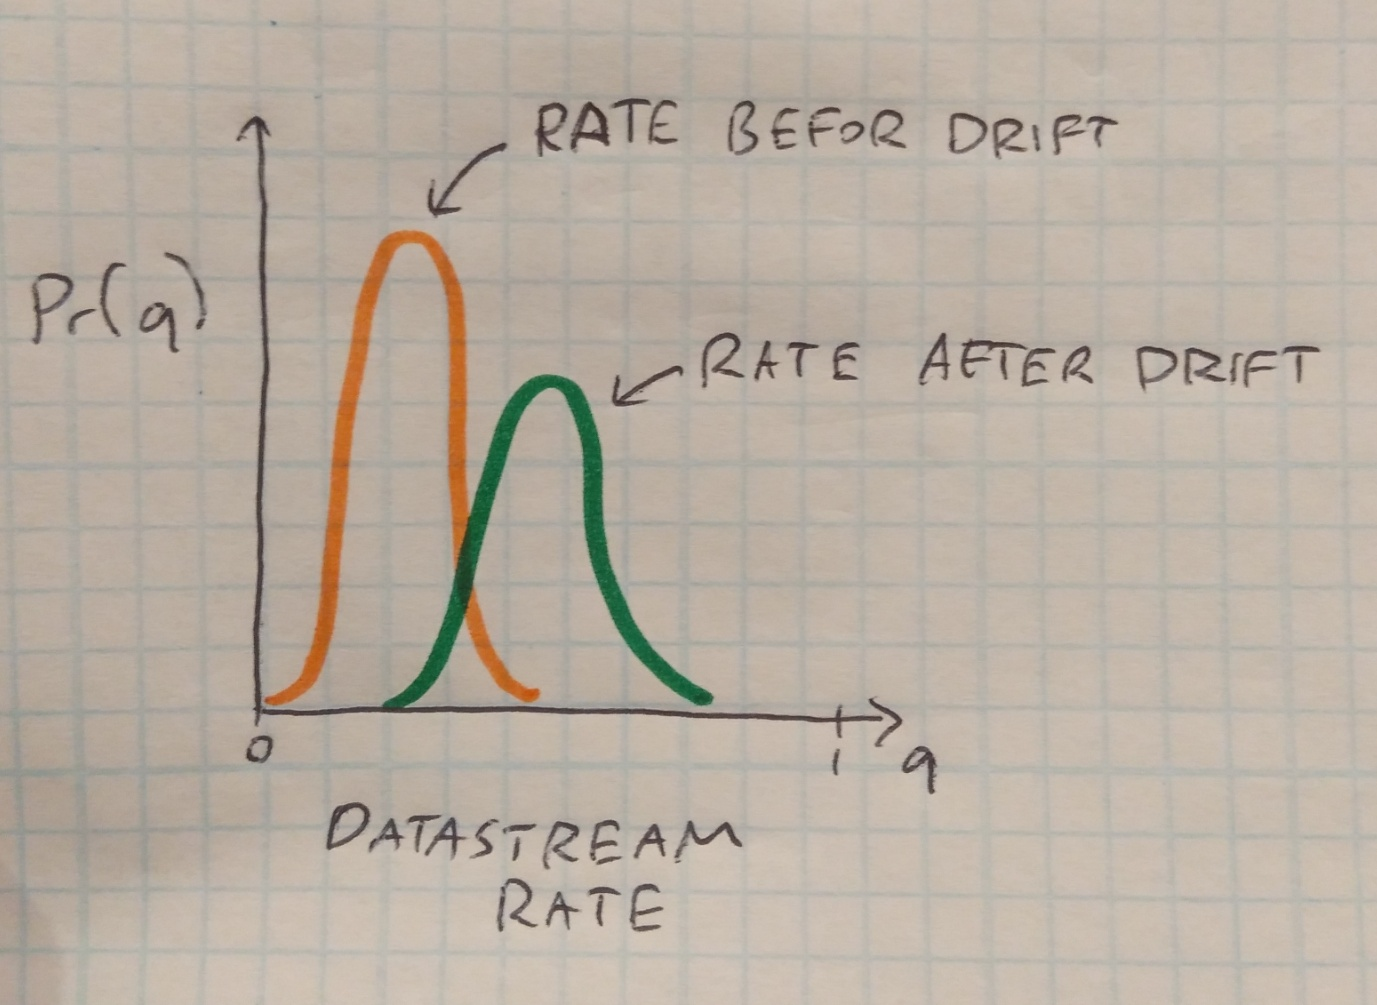
\includegraphics[width=.5\columnwidth]{images/posterior_rates.jpg}
    \caption{Posterior distribution over the original and current error rates of the model when concept drift has occurred.}
    \label{fig:posterior_rates}
\end{figure}



\pgfmathdeclarefunction{gauss}{2}{%
  \pgfmathparse{1/(#2*sqrt(2*pi))*exp(-((x-#1)^2)/(2*#2^2))}%
}
\def\cdf(#1)(#2)(#3){0.5*(1+(erf((#1-#2)/(#3*sqrt(2)))))}%
% to be used: \cdf(x)(mean)(variance)

\begin{figure}
    \centering
    \subfigure[Probability mass function]{
        \begin{tikzpicture}
            % pdf
            \begin{axis}[
                xmin=0,
                xmax=100,
                ymin=0,
                no markers,
                ylabel={$\Pr(d=t)$},
                xlabel=$t$,
                domain=0:100, 
                samples=100,
                width=0.6\textwidth,
                height=0.3\textwidth
            ]
                \addplot {gauss(40,10)};
            \end{axis}
        \end{tikzpicture}
    }
    \subfigure[Cumulative mass function]{
        \begin{tikzpicture}
            % cdf
            \begin{axis}[
                xmin=0,
                xmax=100,
                ymin=0,
                no markers,
                ylabel={$\Pr(d\le t)$},
                xlabel=$t$,
                domain=0:100, 
                samples=100,
                width=0.6\textwidth,
                height=0.3\textwidth,
            ]
                \addplot[smooth,red] gnuplot{\cdf(x)(40)(10)};
            \end{axis}
        \end{tikzpicture}
    }
    \caption{Probability mass function and cumulative mass function over times at which a concept drift may have occurred.}
    \label{fig:bayes_pdf}
\end{figure}

%-------------------------------------------------------------------
% BDDM
%-------------------------------------------------------------------

\section{Bayesian Drift Detection Method} \label{BDD:bddm}

In this section we introduce the Bayesian drift detection method (BDDM). BDDM precisely computes posterior distributions over drift points, as well as the error rates at the start and end of the time series. It is therefore more precise than other drift detectors, but at the cost of having $O(t^2)$ time complexity and $O(t)$ space complexity. %We also present a windowed version which is linear in time and constant in space.

\subsection{Setting}

We pose the problem of computing a posterior over drift points as follows. Given a Bernoulli time series 
\begin{equation}
    Z=z_0,z_1,\dots,z_t
\end{equation}
we would like to compute the probabilities that the rate of the series changed at each time step, as well as the probability no change occurred. The time series in question is the series of residuals of the model. A change in the rate of this series indicates that the error rate has changed which indicates drift. This is the same strategy as used by most other drift detectors \cite{DDM}\cite{ADWIN}\cite{BCMC}, and is referred to as the described as the accuracy-operationalisation in Chapter \ref{chapt:Background}.

We denote the probability that a drift occurred at time step $i$ as $\Pr(d=i)$. Specifically, $\Pr(d=i)$ is the prior probability. For convenience, we denote the probability that no drift has occurred as $\Pr(d=0)$. The posterior probability is the probability of drift conditioned on the observed time series, denoted $\Pr(d=i|Z)$. 

We can express the posterior probability of drift at a given time step using Bayes' rule:
\begin{align}
  \Pr(d=i|Z) &= \frac{\Pr(Z|d=i)}{\Pr(Z)}\Pr(d=i) \\
  &= \frac{\Pr(Z|d=i)}{\sum_{j=0}^t\Pr(Z|d=j)\Pr(d=j)}\Pr(d=i) \label{eq:posterior}
\end{align}
For convenience, we will denote the joint probability of a given sequence with a given drift point as
\begin{align}
  P_i &= \Pr(Z, d=i) \\
  &= \Pr(Z|d=i)\Pr(d=i).
\end{align}
The posterior probability that drift has occurred is given by
\begin{align}
  \Pr(d=0|Z) = \frac{\sum_{i=1}^t P_i}{\sum_{i=0}^t P_i}.
\end{align}

\subsection{Priors}

We require a method for setting unitary priors on possible drift points.
\begin{equation}
  \sum_{i=0}^t \Pr(d=i) = 1
\end{equation}
We propose two systems of priors for BDDM, one for evenly spaced time series and one for unevenly spaced time series. Our motivating example of GP referrals triage is an example of an unevenly spaced time series as GP referral documents or clinician labels can arrive at any time.

A natural prior for evenly spaced time series is a geometric distribution \cite{fearnhead}\cite{BCMC}. We suppose that there is a constant rate of concept drift, and that drift may only occur once. This produces the prior %This is akin to modelling occurrence or non-occurrence of concept drift as a coin flip.
\begin{equation}
  \Pr(d=i) = \begin{cases}
  (1-\lambda)^t & \text{if }i=0 \\
  (1-\lambda)^{d-1}\lambda & \text{if }i>0
  \end{cases}
\end{equation}
where $\lambda \in [0,1]$ is the drift rate, which is the only parameter of BDDM.

We can generalise this strategy to unevenly spaced time series by modelling drift as a Poisson process. Again, we have a ``rate" of drift, but now the rate is per unit time rather than per time step.
\begin{align}
  \Pr(d=i) &= \begin{cases}
  P[N(\tau_t)=0]& \text{if }i=0 \\
  P[N(\tau_{i-1})=0]P[N(\tau_i)>0] & \text{if }i>0
  \end{cases} \\
  &= \begin{cases}
  e^{-\lambda\tau_t} & \text{if }i=0 \\
  e^{-\lambda \tau_{i-1}}\left(1-e^{-\lambda(\tau_i-\tau_{i-1})}\right) & \text{if }i>0
  \end{cases} \\
  &= \begin{cases}
  e^{-\lambda\tau_t} & \text{if }i=0 \\
  e^{-\lambda \tau_{i-1}} - e^{-\lambda \tau_i} & \text{if }i>0 \label{eq:prior}
  \end{cases}
\end{align}
where $\lambda > 0$ is the drift rate, $\tau_i$ is the time at which the $i$-th value arrives, and $N(\tau)$ is the number of drifts which have occurred at time $\tau$. Note that if the instances are evenly spaced in time then this is equivalent to the geometric prior.

\subsection{Likelihoods}

Suppose the error rate of the model $x$ is drawn from a uniform distribution over $[0,1]$. Then the probability of observing a given sequence of residuals is given by the beta function.
\begin{align}
  \Pr(Z; x) &= \int_0^1 x^{\sum_{i=0}^t z_i}(1-x)^{\sum_{i=0}^t (1-z_i)} dx \\
  &= B\left(1+\sum_{i=0}^t z_i,1+\sum_{i=0}^t (1-z_i)\right) \\
  &= \frac{\left(\sum_{i=0}^t z_i\right)! \left(\sum_{i=0}^t (1-z_i)\right)!}{(n+1)!}
\end{align}
where $B(a,b)$ is the beta function.

We assume that if concept drift occurs, the error rates for before and after the drift are drawn independently. Thus
\begin{align}
  \Pr(Z|d=k) &= \Pr(Z_{0:k-1})\Pr(Z_{k:t}) \\
  &= B\left(1+\sum_{i=0}^{k-1} z_i,1+\sum_{i=0}^{k-1} (1-z_i)\right) B\left(1+\sum_{i=k}^t z_i,1+\sum_{i=k}^t (1-z_i)\right). \label{eq:likelihood}
\end{align}

\subsection{Pseudocode}

By combining the priors from Equation \ref{eq:prior} and likelihoods from Equation \ref{eq:likelihood} into Equation \ref{eq:posterior}, we obtain the posterior probabilities of drift at each time step. BDDM is a straightforward computation of this equation, as shown in Algorithm \ref{alg:bddm}. Clearly, BDDM is $O(t^2)$ in time complexity and $O(t)$ in space complexity. %We can impose a limit on the resource requirements of BDDM by only considering the most recent $N$ instances as possible drift points. This is achieved by maintaining a sliding window of size $N$, and reduces the time complexity to $O(tN)$ and the space complexity to $O(N)$. The sliding window version of BDDM is given in Algorithm \ref{alg:bddm_win}.

\begin{algorithm}
    \caption{BDDM algorithm}
    \label{alg:bddm}
    \begin{algorithmic}
        \Require Drift rate $\lambda$
        \Require Warning threshold $\alpha_{warn}$
        \Require Drift threshold $\alpha_{drift}$
        \For {$t=0,1,2,\dots$}
          \State $c_t \gets (z_t, 1-z_t)$
          \Comment We store $z$ values in dummy vectors.
          \For {$k=0,1,2,\dots,t$}
            \State $P_i \gets B\left(1+\sum_{i=0}^{k-1}c_i\right) B\left(1+\sum_{i=k}^t c_i\right) \Pr(d=\tau_k;\lambda)$
          \EndFor
          \State $P(drift) \gets \frac{\sum_{i=1}^t P_i}{\sum_{i=0}^t P_i}$
          \If {$P(drift)>\alpha_{warn}$}
            \State {\tt status} $\gets$ {\tt warning}
          \ElsIf {$P(drift)>\alpha_{drift}$}
            \State {\tt status} $\gets$ {\tt drift}
          \EndIf
        \EndFor
    \end{algorithmic}
\end{algorithm}

% \begin{algorithm}
%     \caption{Sliding window BDDM.}
%     \label{alg:bddm_win}
%     \begin{algorithmic}
%         \Require Window size $N$
%         \Require Drift rate $\lambda$
%         \Require Warning threshold $\alpha_{warn}$
%         \Require Drift threshold $\alpha_{drift}$
%         \For {$t=0,1,2,\dots$}
%           \If {$t<N$}
%             \State $c_t \gets (z_t, 1-z_t)$
%             \Comment We store $z$ values in dummy vectors.
%             \State $\hat{\tau}_t \gets \tau_t$
%           \Else
%             \State $c_0 \gets c_0 + c_1$
%             \State $\hat{\tau}_0 \gets \hat{\tau}_1$
%             \For {$i=1,2,\dots,N-2$}
%               \State $c_i \gets c_{i+1}$
%               \State $\hat{\tau}_i \gets \hat{\tau}_{i+1}$
%             \EndFor
%             \State $c_{N-1} \gets (z_t, 1-z_t)$
%             \State $\hat{\tau}_{N-1} \gets \tau_t$
%           \EndIf
%           \For {$k=0,1,2,\dots,\min(t,N-1)$}
%             \State $P_i \gets B\left(1+\sum_{i=0}^{k-1}c_i\right) B\left(1+\sum_{i=k}^t c_i\right) \Pr(d=\hat{\tau}_k;\lambda)$
%             \Comment Where $1$ is a two-dimensional vector.
%           \EndFor
%           \State $P(drift) \gets \frac{\sum_{i=1}^t P_i}{\sum_{i=0}^t P_i}$
%           \If {$P(drift)>\alpha_{warn}$}
%             \State {\tt status} $\gets$ {\tt warning}
%           \ElsIf {$P(drift)>\alpha_{drift}$}
%             \State {\tt status} $\gets$ {\tt drift}
%           \EndIf
%         \EndFor
%     \end{algorithmic}
% \end{algorithm}

\subsection{Comparison with other Drift Detectors}

BDDM is closely related, but distinct, from other Bayesian approaches to concept drift detection and change point detection. The only other Bayesian method which is intended to be directly applied to machine learning on volatile data streams is BCMC \cite{BCMC}. However, this algorithm requires maintaining an ensemble of one model per potential drift point, and so is too computationally expensive for many applications. The work of Adams and MacKay \cite{adams_mackay}, Barry and Hartigan \cite{barry_hartigan}, and Fearnhead \cite{fearnhead} are concerned with the more general problem of Bayesian multiple change-point detection in data streams, and so cannot be directly applied to our problem.

Modelling drift in a Bayesian manner has many advantages compared to other drift detection methods. By encoding information about time intervals in our priors, we can apply drift detection to both unevenly spaced time series and evenly spaced time series, a feature which most other drift detectors do not possess \cite{sedanspot}. This allows the Bayesian calculations to have more common sense behaviour, such as assigning a higher probability to a concept drift occurring between consecutive instances separated by one day, than consecutive instances separated by one hour.

Another advantage of BDDM is that it does not require parameter tuning. The only parameter is the rate of drift used to calculate priors. This has an intuitive meaning, and its approximate magnitude should be apparent in most domains. This is particularly important in concept drift detection, as we often do not have annotated historical data for parameter tuning. There are few other drift detectors which have such simple parameters \cite{DDM}\cite{CUSUM}. Other drift detectors require tuning thresholds \cite{ADWIN}\cite{HDDM}, window sizes \cite{STEPD}\cite{PL}, or decay rates \cite{HDDM}\cite{EWMA}, which do not have intuitive meanings. %The windowed version of BDDM is not a parameter {\it per se}, and should simply be set according to the computational resources available.

Because we are assigning precise probabilities to each candidate drift point, we can graphically plot the probability mass function (PMF) and cumulative mass function (CMF) of concept drift, as shown in Figure \ref{fig:bayes_pdf}. This makes the drift detector more interpretable. Plotting a PMF or CMF is possible in principle for other drift detectors which explicitly test several candidate drift points, such as ADWIN \cite{ADWIN} and SEED \cite{SEED}. However, because these detectors use frequentist statistics and bound probabilities rather than estimating them, these distributions would be imprecise and non-unitary.

Another benefit of assigning probabilities to candidate drift point is it allows us to model the posterior distribution over the rates of Bernoulli streams before and after the drift point. The posterior distribution over rates in a stable Bernoulli time series is given by the beta distribution.
\begin{align}
  \Pr(q|Z) &= \frac{ x^{\sum_{i=0}^t z_i}(1-x)^{\sum_{i=0}^t 1-z_i} }{B\left(1+\sum_{i=0}^t z_i,1+\sum_{i=0}^t 1-z_i\right)} \label{eq:rate_posterior}
\end{align}
where $q$ is the rate of the Bernoulli stream (the error-rate). Thus, the pre-drift posterior distribution over rates can be calculated from a sum of beta distributions, weighted by the posterior probabilities of each drift point.
\begin{align}
  \overrightarrow{\Pr}(q) &= P_0 \Pr(q|Z_{0:t}) + \sum_{i=1}^t P_i \Pr(q|Z_{0:i-1}).
\end{align}
We can similarly derive the post-drift posterior distribution over rates.
\begin{align}
  \overleftarrow{\Pr}(q) &= \sum_{i=0}^t P_i \Pr(q|Z_{i:t}).
\end{align}
An illustration of these posterior distributions is given in Figure \ref{fig:posterior_rates}. These posterior distributions add to the interpretability of BDDM, and allow retraining decisions to be made on the basis of expected utility.

\begin{figure}
    \centering
    \subfigure[Early stage]{
        \centering
        \resizebox{0.45\textwidth}{!}{
            \bwafFig{6}{20}{4}{13}{30}{45}{45}{20}
        }
    }
    \subfigure[Pre-drift]{
        \centering
        \resizebox{0.45\textwidth}{!}{
            \bwafFig{20}{80}{4}{13}{25}{60}{40}{20}
        }
    }
    \subfigure[Immediate post-drift]{
        \centering
        \resizebox{0.45\textwidth}{!}{
            \bwafFig{20}{80}{10}{15}{25}{60}{50}{30}
        }
    }
    \subfigure[Later post-drift]{
        \centering
        \resizebox{0.45\textwidth}{!}{
            \bwafFig{20}{80}{40}{60}{25}{90}{45}{70}
        }
    }
    \caption{Progression of BWAF algorithm.}
    \label{fig:bwaf_progress}
\end{figure}

%-------------------------------------------------------------------
% BWAF
%-------------------------------------------------------------------

\section{Bayes With Adaptive Forgetfulness} \label{BDD:BWAF}

We now introduce Bayes With Adaptive Forgetfulness (BWAF). This is a drift detector which uses a simple heuristic update rule to approximate the behaviour of BDDM. BWAF is very efficient: it is $O(1)$ space complexity and $O(t)$ in time complexity. 

\subsection{Amnesiac Distributions}

From the Equation \ref{eq:rate_posterior}, we saw that:
\begin{equation}
    \Pr(q|Z) \propto \prod_{i=0}^t x^{z_i}(1-x)^{1-z_i}.
\end{equation}
or in log form
\begin{equation}
    \ln\left(\Pr(q|Z)\right) \propto \sum_{i=0}^t z_i z\ln(x) + \sum_{i=0}^t (1-z_i)\ln(1-x).
\end{equation}
In this formulation, it is natural to think of the posterior as accumulating update terms from each new observed value. We wish to estimate the current rate of the Bernoulli series at time $t$. Because drift may have occurred at any point in the past, we should give greater weights to the more recent updates. A natural way to do this is with exponentially decaying weights. Hence, we can heuristically estimate the posterior distribution over rates as:
% \begin{align}
%     \ln\left(P(q|Z)\right) \propto \sum_{i=0}^t \gamma^{t-i} (1-z_i)\ln(1-x) + \sum_{i=0}^t \gamma^{t-i} z_i z\ln(x) \label{eq:horse}
% \end{align}
% or in the sporadic interval case
\begin{align}
    \ln\left(\overleftarrow{\Pr}(q|Z)\right) \propto \sum_{i=0}^t \gamma^{\tau_t-\tau_i} (1-z_i)\ln(1-x) + \sum_{i=0}^t \gamma^{\tau_t-\tau_i} z_i z\ln(x) \label{eq:horse}
\end{align}
where $0\le\gamma\le 1$ is the {\bf forgetfulness parameter}. Converting this back out of log form gives
\begin{equation}
    \overleftarrow{\Pr}(q|Z) \propto \prod_{i=0}^t (1-x)^{(1-z_t)\gamma^{\tau_t-\tau_i}} \prod_{i=0}^t x^{z_t\gamma^{\tau_t-\tau_i}}.
\end{equation}
Which can be expressed more compactly as
\begin{equation}
    \overleftarrow{\Pr}(q) = \frac{x^a (1-x)^b }{B(a+1,b+1)} \label{eq:banana}
\end{equation}
with
\begin{align}
    a &= \sum_{i=0}^t z_t\gamma^{\tau_t-\tau_i} \\
    b &= \sum_{i=0}^t (1-z_t)\gamma^{\tau_t-\tau_i}.
\end{align}
Thus the current posterior distribution over rates at time $t$ can be derived from Equation \ref{eq:banana} and the following update rules
\begin{align}
    a_t &= \begin{cases} 
        z_t & \text{if $t=0$} \\ 
        z_t + \gamma^{\tau_t-\tau_{t-1}} a_{t-1} & \text{if $t>0$} 
    \end{cases} \\
    b_t &= \begin{cases} 
        (1-z_t) & \text{if $t=0$} \\ 
        (1-z_t) + \gamma^{\tau_t-\tau_{t-1}} b_{t-1} & \text{if $t>0$} 
    \end{cases}
\end{align}
We call this PMF the retrograde amnesiac distribution, as it ``forgets" about about older values from the time series.

We now wish to estimate the initial rate of the Bernoulli stream. Naturally, we should use the opposite weighting scheme as for the retrograde amnesiac distribution. This can be easily achieved with
\begin{equation}
    \overrightarrow{\Pr}(q) = \frac{x^{A-a} (1-x)^{B-b}}{B(A-a+1,B-b+1)} \label{eq:banana_two}
\end{equation}
where
\begin{align}
    A &= \sum_{i=0}^t z_t \\
    B &= \sum_{i=0}^t (1-z_t).
\end{align}
These have the update rules:
\begin{align}
    A_t &= \begin{cases} 
        z_t & \text{if $t=0$} \\ 
        z_t + A_{t-1} & \text{if $t>0$} 
    \end{cases} \\
    B_t &= \begin{cases} 
        (1-z_t) & \text{if $t=0$} \\ 
        (1-z_t) + B_{t-1} & \text{if $t>0$} .
    \end{cases}
\end{align}
We call this PMF the anterograde amnesiac distribution, as it forgets about about {\it recent} values of the time series.

\subsection{Adaptive Forgetfulness}

With posterior distributions over the initial rate and current rate of the Bernoulli stream, we can compute the probability that the rate has increased. 
\begin{align}
    \Pr(q_t > q_0) &= \int_0^1 \overrightarrow{\Pr}(q_0) \int_{q_0}^1 \overleftarrow{\Pr}(q_t) ~dq_t ~ dq_0.
\end{align}
We call this the {\bf drift probability}. If the drift probability exceeds some critical threshold, BWAF will signal that drift has occurred.

% Let $q_t$ be the rate of $z$ at time $t$, and $\bar{q}_t$ be the mean value of $q_i$ for $i=0,1,\dots,t$. $\Pr_B(q)$ gives a posterior distribution of $\bar{q}_t$, and $\Pr_{FB}(q)$ gives a posterior distribution over $q_t$. With this we can perform a one-tailed test for the hypothesis that $q_t \ne \bar{q}_t$. If it is indeed the case that $q_t \ne \bar{q}_t$, then drift has occurred.
% \begin{align}
%     \Pr(q_t > \bar{q}_t) &= \int_0^1 \Pr_B(q = x) \int_x^1 \Pr_{FB}(q = u) du dx
% \end{align}
% The test for the other tail is
% \begin{align}
%     \Pr(q_t < \bar{q}_t) &= \int_0^1 \Pr_B(q = x) \int_0^x \Pr_{FB}(q = u) du dx.
% \end{align}

How do we choose the forgetfulness parameter? We face a trade-off: if the parameter is small then the retrograde amnesiac distribution is more forgetful. This allows it to shift to a new distribution more quickly, and thus have a shorter detection delay. But it also means that it never remembers enough data to know the current rate with much precision. That is, the entropy of the posterior distribution will always be quite high. Thus, small changes in the rate will never be detected.

A good way to get around this problem is to dynamically adjust the forgetfulness parameter. When the drift probability is large, we want the retrograde amnesiac to be updated much more than the anterograde amnesiac. Thus the forgetfulness parameter should increase with the drift probability. The simplest way to achieve this is with the following update rule
\begin{equation}
    \gamma \gets \begin{cases}
        0.5 & \text{when }t=0 \\
        \Pr(q_t > q_0) & \text{when }t>0
    \end{cases}
\end{equation}

The progression of the anterograde and retrograde amnesiac distributions is illustrated in Figure \ref{fig:bwaf_progress}. If no drift has occurred, the anterograde amnesiac distribution will converge towards the current rate. The retrograde amnesiac distribution will oscillate around the current rate, and the drift probability will oscillate around 0.5. The retrograde amnesiac distribution will thus remain high-entropy. When drift occurs, the the drift probability will increase. The forgetfulness parameter will also increase, allowing the retrograde amnesiac to converge towards the current distribution while the anterograde amnesiac continues to estimate the original distribution, thereby further increasing the forgetfulness parameter. The drift probability and the forgetfulness parameter will continue to mutually reinforce one another, until the drift probability reaches the critical threshold. 

The pseudocode for the full BWAF procedure is given in Algorithm \ref{alg:bwaf}

\subsection{Comparison with Other Drift Detectors}

BWAF retains several of the advantages of BDDM. It retains the ability to view the posterior distribution over the current and initial rates of the Bernoulli stream. It does not retain the ability to plot a PMF or CMF of drift occurring, although one can create a diagram analagous to a CMF by plotting the drift probability over time. BWAF is therefore not as interpretable than BDDM, but is still more interetable than most drift detectors. 

As with BDDM, BWAF can accomodate unevenly spaced time series. The choice of units for these intervals will affect the performance of BWAF, and choosing appropriate units is not straightforward. One might adopt the heuristic that the units should be such that the mean interval is one, so that BWAF will behaviour similarly with unevenly spaced time series and evenly spaced time series. 

A major advantage of BWAF is that it does not have any parameters. By dynamically adjusting the forgetting parameter it can in principle detect drifts of any magnitude or any level of abruptness. It is not clear if the same is true of any other drift detectors. DDM has no parameters, but cannot detect drifts which are small compared to sigma \cite{DDM}. In this respect, BWAF is superior even to BDDM, which has the drift rate parameter. As aforementioned, in the case of unevenly spaced time series there is an implicit parameter in the choice of interval units. %However, given that other drift detectors do not even accommodate unevenly spaced time series, the point still goes to BWAF. 

% Further advantages of BWAF are that it is relatively simple and easy to understand, it can be easily adapted to detect drift in both directions, and that it is extremely memory efficient, only requiring four registers. 

It is interesting to note that BWAF has parallels with many disparate approaches to drift detection. The Bayesian connection has already been mentioned. Like DDM and EDDM, BWAF derives p-values from changes in the distribution over the rates of Bernoulli series \cite{DDM}\cite{EDDM}. Similar to ADWIN, a parameter of the model adapts online depending on drift conditions \cite{ADWIN}. Finally, the exponential decay of distribution updates is very similar to EWMA \cite{EWMA}. 

\begin{algorithm}
    \caption{BWAF algorithm}
    \label{alg:bwaf}
    \begin{algorithmic}
        \Require Warning threshold $\alpha_{warn}$
        \Require Drift threshold $\alpha_{drift}$
        \State $\gamma \gets 0.5$
        \State $a,b,A,B \gets 0,0,0,0$
        \For {$t=0,1,2,\dots$}
          \State $a \gets (1-z_t) + \gamma^{\tau_t-\tau_{t-1}} a$
          \State $b \gets z_t + \gamma^{\tau_t-\tau_{t-1}} b$
          \State $A \gets (1-z_t) + A$
          \State $B \gets z_t + B$
          \State $\Pr(drift) \gets \frac{1}{B(a+1,b+1)B(A-a+1,B-b+1)}\int_0^1 (1-q_0)^{A-a}q_0^{B-b} \int_{q_0}^1 (1-q_t)^aq_t^b ~dq_t ~ dq_0$
          \State $\gamma \gets \Pr(drift)$
          \If {$\Pr(drift)>\alpha_{warn}$}
            \State {\tt status} $\gets$ {\tt warning}
          \ElsIf {$\Pr(drift)>\alpha_{drift}$}
            \State {\tt status} $\gets$ {\tt drift}
          \EndIf
        \EndFor
    \end{algorithmic}
\end{algorithm}

%-------------------------------------------------------------------
% CONCLUSION
%-------------------------------------------------------------------

\section{Conclusion} \label{BDD:conclusion}

In this chapter we have introduced BDDM, a drift detector which computes exact posterior probabilities of drift. We have also introduced BWAF, a heuristic drift detection method inspired by BDDM. These detectors offer many advantages compared to other drift detectors. They accommodate unevenly spaced time series as well as evenly spaced time series. They simplify the task of parameter tuning. They are also more transparent than other drift detectors. %These detectors help bridge the gap between concept drift detection research and practical data science by providing solutions to some of the problems which come up in real applications which other drift detection methods are unprepared to deal with.

For future research, it would be useful to theoretically explore BWAF. Can performance guarantees be obtained? Are there different heuristics for updating the forgetfulness parameter which work as well or better?